\documentclass[12pt, a4paper]{article}
%\usepackage{natbib}
\usepackage{cite}
\usepackage{amsmath,amssymb,amsfonts}
\usepackage{algorithmic}
\usepackage{graphicx}
\usepackage{textcomp}
\usepackage{xcolor}
\usepackage[inkscapeformat=pdf]{svg}
\usepackage[inline]{enumitem}
\usepackage[hidelinks]{hyperref}

\usepackage{myacronyms}
\usepackage{listings}
\usepackage{todonotes}
\newcommand{\note}[3]{\todo[inline,linecolor=#1,backgroundcolor=#1!25,bordercolor=#1]{\textbf{#2:} #3}}
\newcommand{\angela}[1]{\note{blue}{Angela}{#1}}

\newenvironment{inlinelist}{\begin{enumerate*}[label=\emph{(\roman*)}]}{\end{enumerate*}}

\usepackage{cleveref}

\begin{document}

%\title{Towards aggregate operating systems with Aggregate Computing}
%\title{Towards collective systems with Aggregate Computing}
\title{Towards collective operating systems through Aggregate Computing}
%\title{Towards collective operative environments with Aggregate Computing}
\author{Angela Cortecchia}
\date{\today}
\maketitle
%
%\setlength{\parindent}{0em}
%\setlength{\parskip}{1em}

% ----------------------------------------
\section{State of the art}
\label{sec:state-of-the-art}
% Esporre sinteticamente lo “stato dell’arte” relativamente al tema di ricerca prescelto,
% con le indicazioni bibliografiche essenziali.
% Se il progetto fa parte di una ricerca più ampia, evidenziare in modo specifico l’attività specifica che ci si propone di svolgere.
% Inserire inoltre gli elementi essenziali utili a dimostrare la coerenza del tema di ricerca prescelto con il percorso di
% formazione e le esperienze pregresse.
%\paragraph{Collective Adaptive Systems}
\sloppypar
\paragraph{Collective Adaptive Systems and Macroprogramming.}
\ac{cas} are systems composed of multiple autonomous entities, such as devices, sensors, and actuators,
that locally interact to achieve a common global goal~\cite{ferscha2015}.
%
These systems adjust to changes in the environment, system requirements, or operational conditions.
%
\ac{cas} are frequently used in \ac{cps} applications where devices collaborate to monitor and control a
physical environment or provide a service to users.

Managing a single device in a distributed system can be challenging for several reasons,
such as \textbf{scalability}, \textbf{device heterogeneity},
\textbf{resource constraints}, and the need to adapt to \textbf{dynamic changes}.
%
Transitioning from a \emph{device-centric} approach,
where the collective is not the abstraction target,
to an \emph{aggregate-centric} approach can lead to various advantages, like
\begin{inlinelist}
    \item distributed intelligence,
    \item resource pooling,
    \item adaptability, and
    \item robustness.
\end{inlinelist}
%
The mentioned challenges can be addressed by using \emph{macroprogramming}.

\emph{Macroprogramming}~\cite{casadei2023} refers
to expressing the macroscopic behavior of a system through a single program using
macro-level abstractions.
%
This approach captures system-level behavior while abstracting individual component interactions.
%
Macroprogramming has been used in different contexts like \ac{wsn}~\cite{1440891}, \ac{iot} applications~\cite{noor19,mizzi18} and swarm robotics~\cite{buzz}.

\sloppypar
\paragraph{Self-organization and Field Calculus.}

Coordination models propose that interaction among multiple independent and autonomous software systems can be designed
orthogonally to pure computation, conceptualized as a shared data space.
%
Over time,
various approaches like \textit{Linda}~\cite{ViroliCoordination2012} and \textit{MARS}~\cite{mars} have emerged,
focusing on centralized local components rather than system distribution.
%
Key challenges in distributed systems include openness to environmental changes, large-scale agent coordination,
and intrinsic adaptiveness to ensure system resilience.
%
Addressing these challenges requires a \emph{self-organization and -coordination} approach,
managing logical interactions to
ensure global and robust coordination behavior.

To facilitate self-organization in complex environments, the \emph{coordination field} concept was introduced as a
navigational tool for agents.
%
The tuple-based middleware \textit{TOTA} (Tuples On The Air)~\cite{tota} supports field-based coordination in pervasive
computing applications.
%
Studies on distributed intelligent systems proposed computational fields for managing space-time
computing models, promoting higher abstractions of spatial collective adaptive systems~\cite{JLAMP2019}.

\ac{fc}~\cite{TOCL2019} emerged as a foundational model for coordinating computational devices in physical environments.
%
\ac{fc} was introduced as minimal core calculus with the aim of capturing the fundaments that make use of computational fields:
functions over and with fields, their evolution over time and the construction of field of values from neighbors.
%
It specifies aggregate system behavior through a dynamic network of directly communicating devices,
using functional compositions of operators manipulating computational fields.
%
Local specifications involve asynchronous computational rounds with three phases:
\begin{inlinelist}
    \item \emph{context building},
    \item \emph{program execution}, and
    \item \emph{export sharing}.
\end{inlinelist}
%
Globally,
\ac{fc} aligns individual device behavior with the network's overarching behavior,
specifying mappings for each device's computation round at space-time events.

\sloppypar
\paragraph{Aggregate Computing/Programming.}
\ac{ap} (or \ac{ac})~\cite{CASADEI2019252} is a functional macroprogramming approach for the compositional development
of self-adaptive \ac{iot} services,
based on the abstractions of \ac{fc}~\cite{MAMEIZL04}.

\ac{ac} programs the behavior of a distributed system by defining interactions among devices as a whole,
rather than individual device behavior,
shifting the fundamental computation unit from a single device to a collaborative group of devices.
%
This structure supports the specification, analysis, simulation,
and runtime execution of \emph{collective} or \emph{aggregate} services,
independently of specific \ac{iot} architectures~\cite{FI2020-pulverization}.
%
The paradigm has three key traits:
\begin{inlinelist}
    \item \emph{global stance with global-to-local mapping}, where the target of system design is the entire distributed \ac{iot} ecosystem,
    \item \emph{service compositionality}, describing rich collective services through the functional composition of simpler services,
    \item \emph{abstraction}, enabling adaptivity by abstracting from low-level details.
\end{inlinelist}
%
These attributes are crucial in both the \emph{design phase},
allowing concise and declarative articulation of complex solutions,
and the \emph{operational phase},
providing flexibility in execution specifics and deployment strategies.
%
Each device of the system locally evaluates the program at a certain frequency,
and communicates with neighboring devices when needed.

\sloppypar
\paragraph{Tools for Aggregate Computing.}

Different tools have been developed to support the \ac{ac} paradigm,
each with its own characteristics and target devices.

\emph{ScaFi (Scala Fields)}\cite{scafi} is a Scala-based framework for aggregate programming,
it provides a \ac{dsl}, libraries, a simulation environment with a GUI,
integrated with the Alchemist simulator~\cite{PianiniJOS2013},
and an actor-based runtime for the development of aggregate computing-based systems.
%
ScaFi is capable of running aggregate programs on the \ac{jvm} and also on web browser thanks to the ScaFi Web tool~\cite{Coordination2021-scafiweb},
which allows the rapid prototyping of aggregate programs.

\emph{Protelis}~\cite{PianiniSAC2015} is a functional programming language that implements a higher-order version of the \ac{fc},
exposed through a C-like syntax,
enabling the construction of widely reusable components of aggregate systems.
%
It also provides various domain-specific APIs that are interoperable with Java, the Protelis-Lang~\cite{SASO2017-protelislang}.
%
Being based on \emph{Xtext},
it necessarily requires a \ac{jvm} to run,
which limits the heterogeneity of devices that can be used in the system.

\emph{FCPP}~\cite{DBLP:journals/scp/AudritoT24} is an implementation of the \ac{fc} as a C++ library,
with tools for simulations of distributed systems.
%
It allows running aggregate programs on low computational capacity devices.
%
However,
its syntax is less ergonomic compared to other languages,
making it unlikely to reach a mainstream developer audience.

\emph{Collektive} is a prototype \ac{dsl} for aggregate computing that extends the \ac{fc} with the \ac{xc}~\cite{AudritoCDSV24},
providing a more expressive language for the development of aggregate systems.
%
This language is more modern and has a user-friendly syntax compared to FCPP and Protelis;
moreover, it is natively multi-platform,
allowing the development of aggregate systems on different devices.

\subsection{Coherence with my previous experiences}
\label{subsec:coherence-with-the-educational-path}

The research project proposed can be seen as an extension of the research activities
carried out with my Master's degree final year and thesis.
%
During the Master's degree,
the exploration of \ac{fc} and \ac{ac} began as a project of the course ``Pervasive Computing''.
%
My project's colleagues and I developed a reimplementation of aggregate computing in Rust,
more specifically the core of the engine inherent to the \ac{fc}.
%
In addition to the development of the engine in Rust,
we also developed a version in Scala 3 of the engine's core that was already implemented in Scala 2,
which is the language used by the ScaFi project.
%
This work provided me with a good foundation in the field of \ac{ac} and \ac{fc}.

The Master's thesis was also focused on the \ac{ac} paradigm.
%
The goal of the thesis was to expand the work done on the Collektive \ac{dsl} previously developed,
by adding the constructs of the \ac{xc} calculus to the language.
%
At the end of the thesis, a prototype of the language was ready and tested on simple case study,
showing the potential of the language in the development of \ac{ac} applications.
%
The thesis therefore helped me to deepen my knowledge of the \ac{ac} paradigm and to understand the potential
of the language in the development of \ac{ac} applications.

During the development of the Master's degree,
I had the opportunity to apply for a research grant that was awarded to me from the \emph{Consortium GARR},
the Italian ``Group for Research Networks Harmonisation'',
and it is currently ongoing.
%
The research grant has the focus on the extension of the work done on the Collektive \ac{dsl},
by creating a standard library of functions that can be used in the development of \ac{ac} applications,
and various demos to show the functionalities of the language.

This experience has allowed me to submit a paper to the \emph{IEEE International Conference on Autonomic Computing and Self-Organizing Systems} (ACSOS 2024),
which is currently under review,
about a generalization of the \emph{Vascular Morphogenesis Controller} (VMC)~\cite{ZahadatHS17} algorithm using the \ac{ac} paradigm.
%
Another paper is currently under submission to the \emph{International Symposium on Distributed Simulation and Real Time Applications} (DS-RT 2024).
%
It is about the development of an architecture and prototype
for monitoring distributed simulations of distributed systems,
where my contribution consists of the development of the simulation used in the evaluation of the architecture,
done using Collektive.

% ----------------------------------------
\section{Project description}
\label{sec:project-description}
\angela{Esporre la finalità della ricerca e descrivere in maniera sintetica la metodologia d’indagine prescelta e la pianificazione sperimentale per perseguire gli obiettivi prefissati.}

\sloppypar
\paragraph{Motivations.}
To coordinate \ac{cas} scenarios in an efficient and effective way,
there is the need to push the abstraction boundaries further than actual existing approaches.
%
This can be achieved by developing a new generation of self-organizing collective systems.
%
Those systems should be able to manage the classical functionalities of an operating system,
such as the management of the devices, the file system, the users, the permissions, and the signals;
while being able to manage the complexity of the environment, the heterogeneity of the devices involved,
and to adapt to the dynamic changes of the environment.
%
The goal of creating a new generation of operating systems based on \emph{collective operating environment}
for opportunistic mobile applications and services is well known in literature,
but few studies have been conducted to effectively develop such systems.
%
Managing multiple concurrent aggregate operations -- where the execution is distributed over space and time
-- poses a significant challenge that is increasingly necessary.
%

Classic aggregate programs are designed to be executed on different devices, independently of external factors;
this could be restrictive in some scenarios.
%
There are situations where the execution of the program should be influenced by external entities,
or where there might be the need to inject processes to inform some devices to execute other tasks,
rather than the one they were executing.

\sloppypar
\paragraph{Research goal.}
The proposed research project aims to investigate the development of \emph{aggregate operating systems},
based on the \ac{ac} paradigm.
%
The project will focus on capturing some of the key features and roles of an operating system with the \ac{ac} paradigm,
such as the management of:
\begin{itemize}
    \item \textbf{collective devices}: combining the capabilities of more devices to achieve a common goal as a single
    entity or logical resource (sensor and actuation fusion);
    \item \textbf{file system}: there are distributed data that should be put together and managed as a single entity,
    there are already some technologies with this aim, but the aim is to get a right level of abstraction to manage the data
    without knowing the underlying technology;
    \item \textbf{users}: groups and sessions that can dynamically adapt to the environment and collaborate between them;
    \item \textbf{permissions}: access to resources and services based on the role of the user relative to the context in which they are located;
    \item \textbf{signals}: the management of the interruption of the processes and the communication between them.
\end{itemize}

Managing those features with the \ac{ac} paradigm allows
writing a single program for the expected behavior of the system,
even if there are different mechanisms behind the various devices involved.
%
In this way,
the software developer does not have to worry about the underlying technology while developing the logic of the system,
allowing for a more abstract and high-level programming approach and to involve heterogeneous devices in the system.
%
The paradigm itself of \ac{ac} offers consistency and resilience to failures,
and the possibility to adapt to \emph{dynamic} changes in the environment.

\sloppypar
\paragraph{Actual functionalities and challenges.}
%
To address the challenges of managing multiple concurrent aggregate operations in a distributed environment,
a system has been developed for managing \emph{aggregate processes}~\cite{aggregate-processes} based on \ac{fc}.
%
Aggregate processes are concurrent field computations
whose execution and interactions are sustained by a dynamic team of devices,
and whose spatial region can opportunistically change over time.
%
This concept captures aggregate behavior, dynamicity and context orientation and intrinsic resiliency;
and as perks, it offers to limit the consumption of computational resources,
maintain a good quality of service,
and enhance the dynamics of distributed computations.

These types of processes differ from the concentrated ones.
%
In particular, there are specific issues that arise in the aggregate approach rather than the traditional one.
%
For example, managing process interruptions, determining the owner of a process and the resources it can access,
or understanding what it means to send a signal to a process.

All of these issues are already resolved in the traditional approach,
but they still need to be investigated and addressed in the aggregate approach.
%
For instance, in the aggregate approach termination is managed collectively.
%
However,
there may be situations where a single device decides to terminate processes or where a process using shared
resources loses the right to use them during execution,
introducing a distributed consensus problem.
%
In practical cases, there may be situations of crowd sensing or crowd steering where,
eventually,
law enforcement realizes that too many people are gathering.
%
Depending on the situation,
these third-party entities can decide to interrupt the crowd-management process.

Another matter not yet addressed is the management of the users in an aggregate environment.
%
There is the need to understand what does it mean to have a user in an aggregate environment,
and how to manage the permissions of the users in the system.
%
Given the features and innovations that the \emph{aggregate processes} approach brings to the field of \ac{ac},
the idea of exploring and expanding the concept on the basis of \emph{aggregate processes} to the development
of a new generation of operating systems arises.

\sloppypar
\paragraph{Example applications.}
An example of application of the system could be in the management of a drone fleet,
where the drones have to collaborate to achieve a common goal,
such as monitoring a specific area,
but the operating system sees them as a single ``sensor'',
in this way the abstraction of the system is higher and the management of the system is easier.

Or even in the management of a smart city,
where the system has to manage the data of the city and the users,
there may be the need to monitor parking lots so a user can find a free one,
or officers can manage the traffic in the city,
or even the system can manage the lighting of the city based on the presence of people in the streets.

% ----------------------------------------
\section{Expected results}
\label{sec:expected-results}
\angela{Descrivere sinteticamente quale apporto la ricerca può fornire all’avanzamento delle conoscenze scientifico-tecnologiche
e le eventuali ricadute sulla società, ponendo in rilievo i profili di originalità dei risultati attesi.
date delle metriche devo trovare un confronto a quelle dove vado a migliorare}

As results of the proposed research project,
it is expected to bring
\begin{inlinelist}
    \item a contribution to the advancement of scientific and technological knowledge in the field of \ac{ac} and \ac{cas},
    \item a formal model of how it should work,
    \item a prototype of the system that is able to manage in a simple and effective way some of the problems that arise in a collective environment.
\end{inlinelist}
%
For instance,
one of the problems presented involves communication between ships in the Kiel Canal
and the amount of data that they can exchange depending on the type of communication available.
%
Specifically,
the farther apart the ships are,
the fewer data they can automatically exchange.
%
Currently,
this issue remains unresolved in an effective manner.
%
Therefore,
it is believed that through \ac{ac},
and particularly through the use of \ac{xc},
a contribution can be made towards solving this problem.

As a long-term vision,
the system will be able to manage many devices in a collective environment,
where the devices can be heterogeneous and can change over time.
%
As seen in ~\Cref{fig:example-of-application},
some of the application scenarios where the system can be used are
\begin{inlinelist}
    \item \emph{smart cities},
    \item \emph{swarm scenarios},
    \item \emph{crowd management},
    \item \emph{morphogenesis},
    \item \emph{autonomous vehicles},
    \item \emph{surveillance}.
\end{inlinelist}

% ----------------------------------------
\section{Subdivision of the project and timeline}
\label{sec:subdivision-of-the-project-and-timeline}
\angela{Illustrare lo sviluppo temporale della ricerca nei 3 anni di progetto, con particolare enfasi sul primo anno.}

\begin{figure}
    \centering
    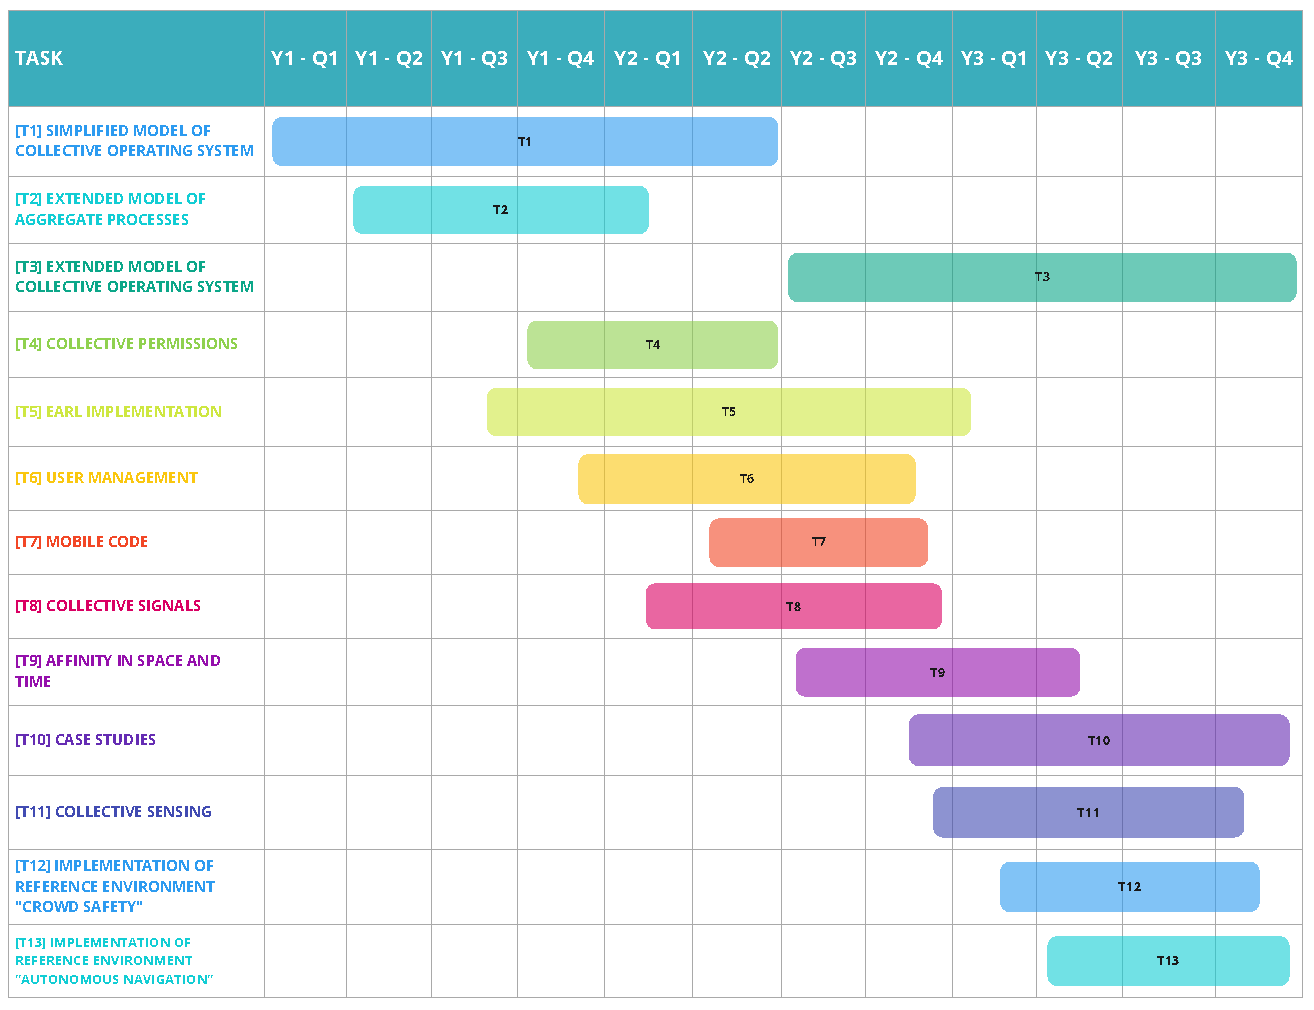
\includegraphics[width=0.9\textwidth]{figures/timeline}
    \caption{Hypothetical timeline of the three years of the project.
        Years are subdivided in quarters, Q1 is from January to March,
        Q2 is from April to June, Q3 is from July to September, and Q4 is from October to December.
    }\label{fig:timeline}
\end{figure}

In the \Cref{fig:timeline} is shown a hypothetical timeline with tasks of the three years of the project,
where each year is subdivided into quarters.

\sloppypar
\paragraph{First year}
In the first year of the project,

it is essential to thoroughly investigate the state of the art and create a simplified model of how the new system should work.
%
Following this,
the actual development process begins with the implementation of the aggregated processes in the target language Collektive.
%
From this foundation,
the development of concepts such as permissions, user management, and signal management can begin,
with these elements being conceptually interconnected.
%
All of this will contribute to the creation of an initial system prototype.

\sloppypar
\paragraph{Second year}
In the second year of the project,
the focus will be on continuing the development of the prototype,
expanding on the concepts investigated in the first year,
and incorporating features such as runtime aggregate programs injection.
%
Towards the end of this period,
the extended model of the Collektive operating system will be drafted,
with a focus on collective sensing of external devices.

\sloppypar
\paragraph{Third year}
In the third year,
use cases will be further investigated,
leading to their actual implementation and testing,
initially in simulated environments and to evaluate performances and effectiveness.

% ----------------------------------------
\section{Proposed evaluation criteria}\label{sec:proposed-evaluation-criteria}
\angela{Descrivere sinteticamente quali modalità si intendono utilizzare durante lo svolgimento del progetto per il monitoraggio
e la valutazione del raggiungimento dei risultati attesi.}
As evaluation criteria,
it can be considered the effective functioning of the system in simulated scenarios,
having a demonstration with heterogeneous devices with the ability to manage a large number of devices,
and at the end of the third year may be considered the possibility of a real-world test with drones or other devices.
%
Furthermore,
it can be used as a metric the amount of scientific contributions that the project brings to ``self-organizing systems'' communities,
such as \emph{ACSOS}\footnote{\url{https://acsos.github.io}} or \emph{SEAMS}\footnote{\url{https://conf.researchr.org/home/seams-2025}},
or even journals such as \emph{ACM TAAS}\footnote{\url{https://dl.acm.org/journal/taas}}.
%
Some practical examples of what the system should be able to do are forcing the termination of a process from an entity with the right permissions,
or effectively injecting code into a process to change its behavior.

% ----------------------------------------
\bibliographystyle{IEEEtran}
\bibliography{bibliography}

\end{document}
